\section{Hardware}

The WWLLN Service Unit uses a Gumstix WaterStormCOM mounted on a Tobi breakout board as the on-board computer to run the WWLLN software.

\subsection{Hardware Summary}

The Gumstix WaterStormCOM is part of the Overo COM series and has the following features:

\begin{itemize}
\item 1~GHz ARM Cortex-A8 CPU
\item 512~MB RAM
\item microSD Card Slot
\item OpenGL POWER SGX graphics Aaccelerator
\item C64x Fixed Point DSP (Max: 660,800~MHz)
\end{itemize}

The Tobi breakout boards adds:

\begin{itemize}
\item HDMI video Out
\item 1 USB port
\item 1 USB console connection
\item Stereo in/out
\item Ethernet
\end{itemize}

\subsection{Pinouts}

The Gumstix COM has direct pinouts to the processor, however as it is not used without the Tobi breakout board, only the Tobi pinout is shown in Figure~\ref{app:gumstix:fig:tobi}.

\begin{figure}[ht!]
   \centering
   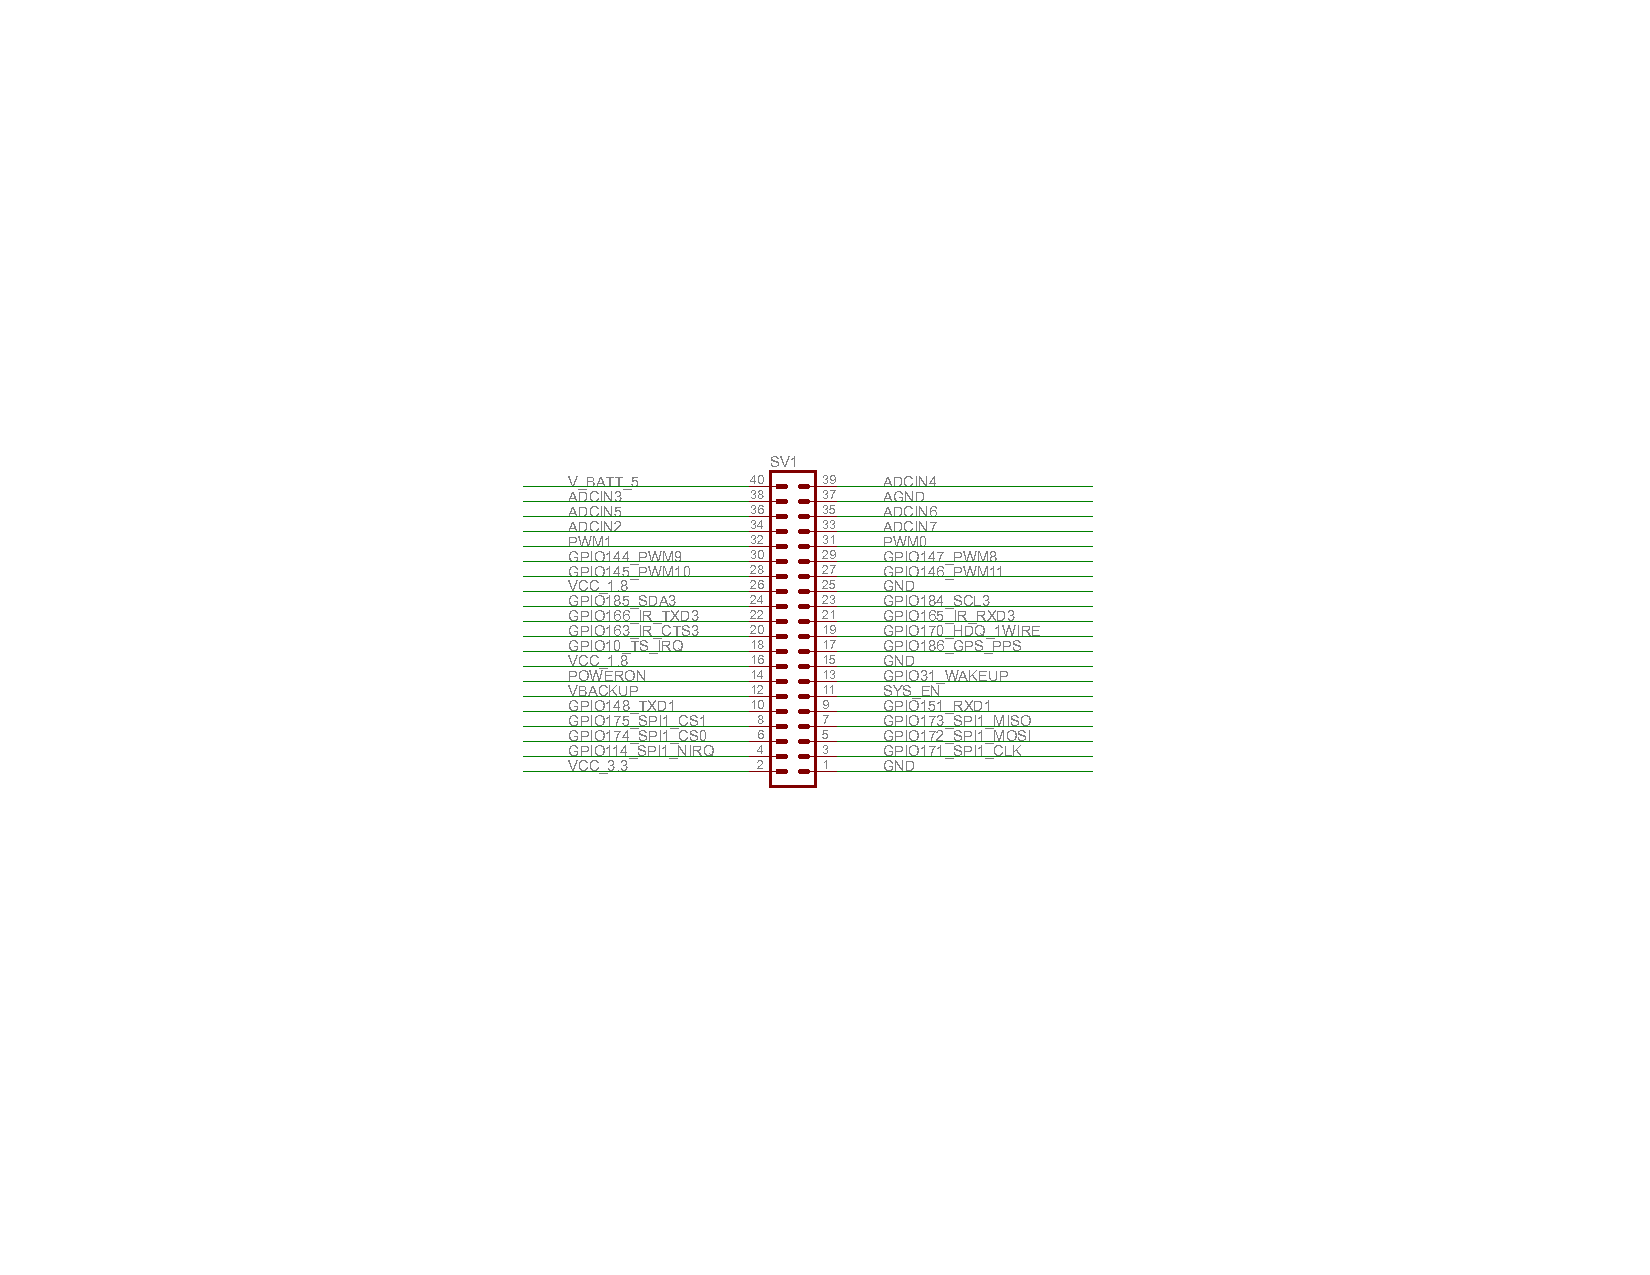
\includegraphics[scale=1]{Appendix/Figures/tobi_pinout.pdf} 
   \caption{Pinout of the Gumstix Tobi breakout board.}
   \label{app:gumstix:fig:tobi}
\end{figure}

In the service unit only pins 1 (GND), 9 (RXD1), 10 (TXD1), 28 (GPIO145), and 40 (V\_BATT) are used.
RXD1 and TXD1 are used for the serial communication with the GPS.
GPIO145 is used to control the pre-amp power supply.
V\_BATT is the 5~V power for the Gumstix.

\section{Gumstix Operating System}

\subsection{\r{A}ngstrom}

The Gumstix used in the service unit is running the basic \r{A}ngstrom operating system (http://www.angstrom-distribution.org).
It also supports Ubuntu, however Ubuntu has been found to be slow and harder to configure with the Gumstix.
\r{A}ngstrom runs similar to most unix operating systems, with the main difference being the opkg package manager instead of yum or apt-get.

A useful resource in setting up and configuring the Gumstix software is the Gumstix developer site (http://gumstix.org) and the mailing list archive forum (http://gumstix.8.x6.nabble.com).

\subsection{Distribution Location}
\label{app:gum:distribution}
The operating system used is the Sakoman GNOME r13 build, available online:

http://www2.sakoman.com/category/8-gnome-daily-builds-r13.html

http://feeds.sakoman.com/feeds/gnome-r13/images/

Or in the /home/mlhutch/Git/gumstix.git repository on flash5 in the baseKernel folder.

\subsection{Bitbake and the Kernel}

The default kernel provided in the builds listed above is missing the ability to run ipfilter which is necessary as the firewall on the Gumstix operating system.
To enable this the kernel needs to be reconfigured to run netfilter, then compiled and deployed.
Bitbake was used previously to alter the linux kernel.

To set up a Bitbake development environment it is recommended to follow a guide such as:
http://ezrover.com/ 2012/01/12/ sakoman-r13-gnome-firmware-howto-101-guide-for-gumstix-overo-openembedded-board/
Where the git repository for the bitbake and recipes is either:
www.sakoman.com/git/openembedded.git
or already pre-configured with the netfilter options on flash5 in the /home/mlhutch/Git/openembedded.git repository.

The following commands allow for changing the kernel:

\begin{enumerate}

\item \begin{verbatim}cd openembedded \end{verbatim}
\item \begin{verbatim}make ARCH=arm menuconfig \end{verbatim}

\item Enable all netfilter options under: Networking Support / Networking Options / Network Packet Filtering (netfilter) /

\item save results as new.config
\item Copy (and backup originals) as defconfig in: recipes/linux/linux-sakoman-pm-3.0/omap3-multi/defconfig

\item \begin{verbatim}bitbake virtual/kernel -c clean \end{verbatim}
\item \begin{verbatim}bitbake virtual/kernel \end{verbatim}

\end{enumerate}

Where the resulting kernel and modules are found in the tmp/deploy/glibc/images/overo/ directory.

After deploying a new kernel it may be necessary to recover the default boot variables on the Gumstix.
On the initial Gumstix startup, pause in the first 5 seconds (this needs to be done via the USB-console connection).
Once paused the defaults can be restored with:

\begin{verbatim}
nand erase 240000 20000
reset
\end{verbatim}

\section{Software}

\subsection{WWLLN Software}

The WWLLN software is provided by James Brundell and compiled specifically for the ARM process.
The three programs are {\bf toga}, {\bf ntpcheck}, and {\bf GDspectro}.
{\bf toga} is the main WWLLN processing programming that reads in the VLF and GPS signals to produce the UDP packets sent on to the main WWLLN processors.
It should be always running on the system with a crontab entry such as:

\begin{verbatim}
0,5,10,15,20,25,30,35,40,45,50,55 * * * * toga -s 100 -a 3 -j 1 -g -o &
\end{verbatim}

This will try to start it every 5 minutes in case it stops for any reason.

The {\bf ntpcheck} and {\bf GDspectro} and programs used by {\bf toga} but do not need to be called or run on their own.

\subsection{Hardware Controls}

Pin GPIO145 is the pin that controls whether the preamp power supply is turned on or off.
When the pin is held low (value of 0) the power supply is on, when it is set high (value of 1) it is turned off.
The command to change a GPIO pin value is:

\begin{verbatim}
echo 0 > /sys/class/gpio/gpio145/value
\end{verbatim}

The two scripts {\bf preampOn.sh} and {\bf preampOff.sh} can be used to easily toggle the preamp power supply.

The default value for GPIO pins is to hold them high, so during boot the preamp turns off until the {\bf preampOn.sh} script can be called at the end of the boot sequence.

\subsection{GPS Interface}

The Trimble GPS communicates with the TSIP protocal, compared the NMEA of the previous GPS engine used.
The pythons script {\bf readTSIP.py} interprets the TSIP messages and reports the GPS status to the file gps.log and prints them to the console.
The console printing can be turned off by changing the variable print\_to\_console to False.

The program can be started and run in the background to produce a continues record of GPS activity.
The default location for the gps.log file is in the public\_html folder where it can be remotely checked through the service unit website.

\subsection{RAM Disk}

The \r{A}ngstrom distribution for Gumstix automatically sets up a RAM disk for users.
It is created at /media/ram with half of the available RAM (256~MB).
It needs to be used for the running of the WWLLN software as the microSD card is too slow.
At start-up the public\_html folder (logs and spectrograms) and sferics folder are created in the ram disk and symlinked to the main sferics directory.

For this reason all permanent edits to the Service Unit website should be made in the public\_html\_static directory.

\section{Creating Gumstix microSD Card}

There are two methods for configuring a new microSD card for use with the service unit Gumstix computer.
Either a card can be formatted and loaded with the latest software using the {\bf makeSD.sh} script and other configuration scripts, or an existing installation disk image can be copied over.

\subsection{Formatting and Installation}

The {\bf makeSD.sh} is based on the script given in Subsection~\ref{app:gum:distribution}.
It is configured to run on a Linux system but may also work with other Unix based operating systems.
The script automatically formats the microSD, loads the bootscripts, loads the operating system, and updates the kernel and modules produced with Bitbake.

\subsection{Installing Packages}

After a card has been successfully partitioned with a new operating system installed it should be run in a Gumstix to allow for the new kernel to configure the necessary modules.
This process takes a few hours for each card, on top of installation, so it is recommended that further cards are created via duplication described below in subsection~\ref{app:gumstix:duplication}.

Once configured a new user can login as {\bf root} with the password {\bf root}.
In the root directory should be a folder called {\bf firstRunFiles}.
The {\bf install.sh} script should be run after connecting the Gumstix to the internet (the script will start dhcp).
This script will install all of the necessary packages for the Gumstix to function as a WWLLN station.

\subsection{Configuring Settings}

With the packages installed the Gumstix needs to be configured with the {\bf setup.sh} script.
The first three tasks of the script are changing the root, sferix, and host passwords.
They should be set according the current standard password practices (contact Robert Holzworth bobholz@ess.washington.edu for exact details).
The script finishes by moving all of the programs, crontabs, startup scripts, bash profiles, and WWLLN programs to the sferix and host accounts.
Lastly it sets up the RAM disk to use with the web server and running the toga program.

\subsection{Card Duplication}
\label{app:gumstix:duplication}

Once a new card is created it is advised to make an exact copy of the card to allow for duplication onto new cards.
Since the partitioning, and bit location on the card, is critical for the Gumstix the direct copy program {\bf dd} should be used to make the copy.
To copy a card to a disk image the command will look like:

\begin{verbatim}
sudo dd if=/dev/sdb of=/Path/To/Target/gumstix.iso bs=512
\end{verbatim}

And the command to copy a microSD image back to a new card in the same slot as the previous card:

\begin{verbatim}
sudo dd if=/Path/To/Target/gumstix.iso of=/dev/sdb bs=512
\end{verbatim}

A word of warning: the {\bf dd} command can overwrite and destroy hard drives if they are incorrectly targeted.
Always double check the mount point of the microSD card before running the {\bf dd} command.

\section{Gumstix System Setup}

Subsection~\ref{app:appendix:setup} gives the setup instructions for a new station, namely setting the IP address so it can be added to the network.
A more up to date version is available in the {\bf gumstix.git} repository in the {\bf user\_manual} folder.
Also included in the station setup instructions are how to setup and customize the service unit webpage, as described in Subsection~\ref{app:gumstix:website}.

\subsection{Connecting to the Gumstix}
\label{app:appendix:setup} 
%%
%% Update to latest version

\subsection*{Method 1: SSH Setup}
The SSH setup method requires:
\begin{itemize}
\item{Ethernet cable}
\item{SSH capable computer}
\end{itemize}

\begin{enumerate}
\item{Connect SU to a host computer directly with an ethernet cable}
\item{Set host computer ethernet network settings to:
\begin{verbatim}
address:	192.168.10.1
gateway:	192.168.10.100
netmask:	255.255.255.0
\end{verbatim}}
\item{SSH into the SU from host computer:
\begin{verbatim}
ssh -p 7777 sferix@192.168.10.2
password: [	]
\end{verbatim}}
\item{Set desired static ip configuration in file $\sim$/networkSetup.sh}
\item{\begin{verbatim}
sudo ./networkSetup.sh
\end{verbatim}}
\item{Switch SU to main network ethernet within 1 minute of running networkSetup.sh}
\item{Test connection by SSH'ing into SU with new IP address}
\item{
\begin{enumerate}
\item{If successful: set new IP setting in /etc/network/interfaces}
\item{If unsuccessful: power cycle SU and check settings starting with step 3}
\end{enumerate}}
\item{Reset SU and confirm new settings}
\end{enumerate}

\subsection*{Method 2: Workstation Setup}
The Workstation setup method requires:
\begin{itemize}
\item{HDMI Monitor and cable}
\item{{\bf Powered} USB Hub}
\item{USB Keyboard}
\item{USB Mouse}
\end{itemize}

Connect the powered USB hub to the back USB port of the service unit, and attach the keyboard and mouse to the hub.
Connect a monitor to the HDMI port, DVI - HDMI adapters work as well.
Power on the box, it will take a few minutes for the login screen to show up.
Select ``Other...'' and login with the username \textbf{host}.
Wait a few more minutes for the graphical display to load.

Adjust the network settings by either changing the files listed in Method 1, or by logging in as root as adjusting them through System $\rightarrow$ Network in the top menu bar.

\begin{enumerate}
\item{Connect an HDMI display, keyboard and mouse}
\item{Set network information through GUI}
\end{enumerate}


\subsection*{Method 3: Manual microSD Editing}

The file that need to be edited on the rootfs partition are:

\begin{verbatim}
/etc/network/interfaces
/etc/resolv.conf
/etc/init.d/dropbear
\end{verbatim}

The interfaces file lists the IP information of the machine whole the resolv.conf file is for the DNS information.
The sshd\_config file on line 13 sets the port with which SSH is allowed.

The last step, if a non-standard port is being used, is to also alter the built in firewall of iptables and netfilter.
The firewall settings are stored in:

\begin{verbatim}
/etc/iptable.rules
\end{verbatim}

and can be edited as a standard iptables configuration file.

\subsection{Website Setup}
\label{app:gumstix:website}

\subsection*{Starting apache2}

To get apache2 running only one change needs to be made in the /etc/apache2/httpd.conf file.

\begin{verbatim}
Line 96:	#ServerName www.example.com:80
\end{verbatim}

Needs to be uncommented and changed to the hostname of the computer, e.g.:

\begin{verbatim}
Line96:	ServerName gumstix.ess.washington.edu:80
\end{verbatim}

Then httpd needs to be restarted:

\begin{verbatim}
sudo httpd -k restart
\end{verbatim}

\subsection*{Setting up the website}

All changes to the website need to be made in the /home/sferix/public\_html\_static folder, this folder is copied to /home/sferix/public\_html during start up. Changes to public\_html are not saves as the folder is located in system RAM due to SD card read/write limitations. A restart in not necessary if the public\_html\_static contents are copied to public\_html.

\subsection{Sound Settings}

The Gumstix a myriad of analog inputs that are all controlled with {\bf alsamixer}.
For the WWLLN service unit the stereo input is controlled by the $<$Analog$>$ input as shown highlighted in Figure~\ref{app:gumstix:fig:alsa}, and a digital gain through $<$TX1 Digital$>$.
Included in the installation files is the default alsa profile {\bf asound.state}.

\begin{figure}[ht!]
   \centering
   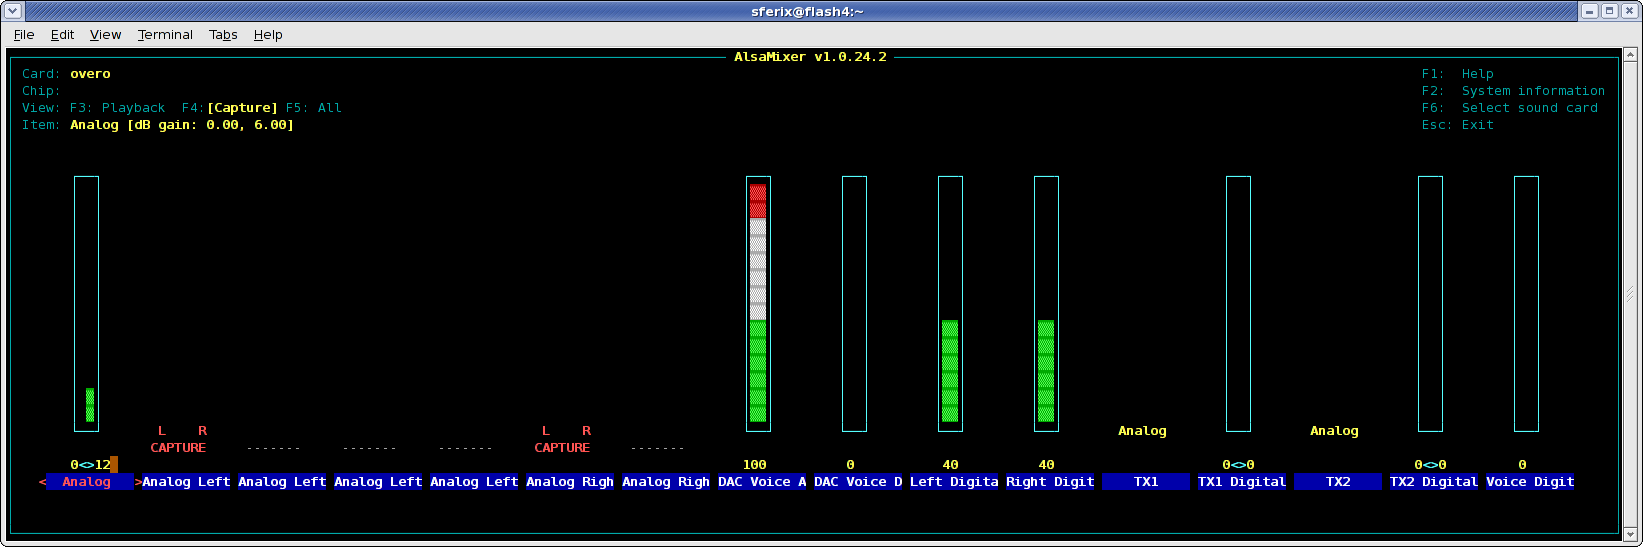
\includegraphics[scale=.3]{Appendix/Figures/gumstixmixer.png} 
   \caption{Alsamixer settings for Gumstix stereo input, $<$Analog$>$ controls the stereo gain.}
   \label{app:gumstix:fig:alsa}
\end{figure}

